\clearpage
\section{Design of CAPS}
\label{sec:design}

Following an overview of \ac{name}'s design (\autoref{sec:design:overview}), we
describe \ac{name} in detail, including how it signals which domains have
deployed \ac{https} and improvements to the Web \ac{pki}
(\autoref{sec:design:signaling}), how it provides stronger public-key
authentication over the existing Web \ac{pki} (\autoref{sec:design:policy}), and
how clients establish secure end-to-end connections with servers
(\autoref{sec:design:handshake}). We conclude by describing how \ac{name} thus
enables the bootstrapping of more advanced policies
(\autoref{sec:design:bootstrapping}).

\subsection{Overview}
\label{sec:design:overview}

\begin{figure*}
  \centering
  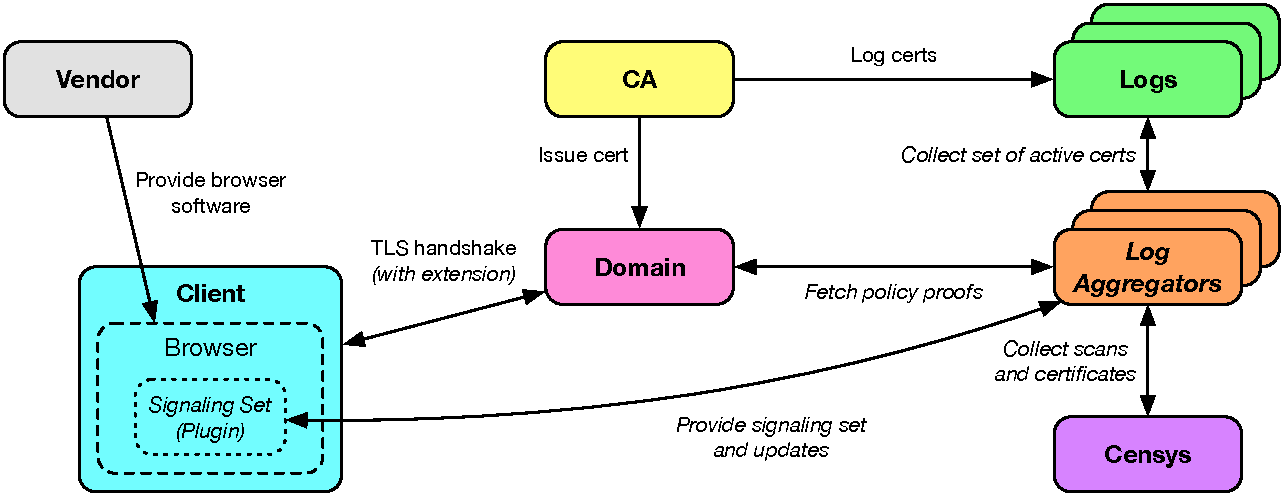
\includegraphics[width=0.8\linewidth]{fig/arch}
  \caption{Overview of \ac{name} architecture (log auditors and monitors not
  shown). Dotted lines denote the browser and its components, and italic text
denotes new entities or actions in \ac{name}.}
  \label{fig:overview}
\end{figure*}

\paragraph{Goals}

\ac{name} primarily aims to enable a smooth transition from the Web's existing
\ac{pki} to an \emph{improved \ac{pki}} (which can range from an extension of
the existing \ac{pki} to a new \ac{pki} altogether). We assume that during this
transition, both the existing and improved \acp{pki} will coexist, and that the
improved \ac{pki} will make \ac{mitm} attacks more difficult to carry out.
Hence, \ac{name} must prevent downgrades to the old \ac{pki}. More precisely, if
a client and server both support the improved \ac{pki}, then when they perform a
handshake, they should negotiate a session key based on the domain's public key
as certified in the improved \ac{pki}. As secondary objectives, we also seek to
prevent domains from becoming inaccessible due to misconfiguration, private key
loss, or private key compromise, and to minimize the changes to existing
interactions between clients, domains, and \acp{ca}.

\paragraph{Adversary Model}

In designing \ac{name}, we consider a \iac{mitm} adversary. 
%We assume the adversary has access to the
%signing keys for $n$ \acp{ca} and can thus issue and revoke arbitrary
%certificates under these keys. 
We assume that the adversary has full
control of the network during the TLS handshake; that is, the adversary can
intercept, drop, or modify all messages sent among all entities described
below. We assume that the adversary cannot mount \iac{mitm} in the improved
\ac{pki}, or break standard cryptographic primitives.

\paragraph{Architecture}

\autoref{fig:overview} illustrates the \ac{name} architecture and how \ac{name}
achieves the goals stated above. Since \ac{name} transitions from the current
Web \ac{pki}, it necessarily includes the entities in the current \ac{pki}:
\begin{compactitem}
\item \emph{Domains} serve webpages to clients. Each domain has a name such as
  \texttt{example.com}.
\item \emph{\acp{ca}} issue certificates to domains. Each certificate binds a
  set of names to a single public key.
\item \emph{Clients} connect to domains over HTTP or \ac{https}, and in the
  latter case, verify the binding between a domain's name and public key.
\item \emph{Browser/OS vendors} (hereafter simply \emph{vendors}) provide the
  software by which clients connect to domains and verify domains' certificates.
\item \emph{Public logs} maintain a publicly auditable, append-only database of
  certificates, such as those used in \ac{ct}.
\end{compactitem}
\ac{name} introduces a new entity, the \emph{log aggregator}, that uses publicly
available data to maintain a database of domains that have deployed \ac{https}
and/or the improved \ac{pki}. As our figure shows, there may be multiple
independent log aggregators. While throughout this section we assume that the
log aggregator is separate from other entities and that there is a globally
accepted set of known and trusted log aggregators, in \autoref{sec:discussion}
we discuss how we can relax these assumptions, namely, by arguing that browser
vendors should take on this responsibility.

% Procedures from the current PKI
As shown in \autoref{fig:overview}, many of the interactions between entities in
the current \ac{pki} remain the same in \ac{name}. \acp{ca} remain entirely unchanged;
they issue certificates
to domains and log newly-issued certificates as they do in the current \ac{pki}
(with \ac{ct}). Clients and domains establish an encrypted communication channel
through the standard \ac{tls} handshake, and vendors provide clients with browser
software.

% Signaling set overview
To prevent an adversary from forcing an HTTP connection (and thus bypassing \ac{tls}
completely), the log aggregators use data from public logs to construct a
\emph{signaling set}, which succinctly represents the set of all domains that
deploy \ac{https}. The log aggregators build this set by downloading the set of
all currently valid (i.e., non-expired) certificates from the logs and
extracting all domains named in these certificates. The log aggregators then
make this set, as well as updates to this set over time, available to client
browsers.  When connecting to a server, the browser first checks whether
the server is in the signaling set; if it is, then the browser will refuse
to accept an HTTP connection.

% Policy overview
To allow domains to certify their public keys more securely than in the current
\ac{pki}, log aggregators use data from public logs to construct a set of
\emph{\ac{name} policies}, which allows each domain to establish an
\emph{authoritative public key} in the \emph{curent} Web \ac{pki}. \ac{name}
policies take a simple and intuitive approach: \emph{treat whichever public key
  is backed by the most independent certificate chains\footnote{This term means
  that the certificate chains share no public keys except at the leaf.} in the
current \ac{pki} as authoritative in the improved \ac{pki}}. A domain wanting to
increase client confidence in one of its public keys can simply obtain more
independent certificates for that key, and the log aggregators will
automatically update their \ac{name} policies for that domain.

Intuitively, log aggregators simply send a signed pair $(\hostname, \policy)$
where \hostname is a domain name and \policy is the \emph{\ac{name} policy
  value}, i.e., the number of independent certificate chains backing an authoritative
  key for \hostname.\footnote{\hostname may have more than one authoritative
  key; if public keys $\pk_1$ and $\pk_2$ are both backed by three independent
chains, for example, then both public keys are treated as authoritative
for \hostname.} To prevent an adversary from downgrading handshakes in the
improved \ac{pki} to a handshake in the existing Web \ac{pki}, each log
aggregator indicates which domains in its signaling set have a key policy value
greater than 1.

The current PKI actually supports two classes of certificates: 
standard ``domain-validated'' (DV) certificates
and
extended validation (EV) certificates.
The latter require domains to undergo more rigorous screening.
Hence, the actual \ac{name} policy value is a tuple $(\policy_{EV}, \policy_{DV})$.
For a given domain, \ac{name} will treat as authoritative the public
key with the largest $\policy_{EV}$, with ties broken based on the largest $\policy_{DV}$.

%Our policy also implies that if $n$ is the
%highest number of observed independent certificate chains for a given domain,
%then \emph{any} public key backed by $n$ chains can be used as that domain's in
%the improved \ac{pki}. Thus, it is possible for a domain to have multiple public
%keys in the improved \ac{pki}.\footnote{In practice, any improved \ac{pki} can
%enforce the use of a single public key by, for example, considering the first
%key backed by $n$ chains as authoritative and using a ``cool-off period'' as in
%AKI~\cite{kim2013accountable}.}


%To move towards \iac{pki} with increased resilience to the compromise of trusted
%parties (i.e., \acp{ca}), we need to prevent \iac{ca} that misissues a
%certificate for a domain from exposing that domain to \iac{mitm} attack. We
%observe that signatures from multiple independent \acp{ca} on a single public
%key can spur greater trust in the key, and therefore we design \ac{name} around
%the idea that domains should be able to obtain and communicate the presence of
%multiple certificates for a single public key. We can then protect domains from
%\ac{mitm} attacks by simply communicating to the client the number of
%certificates to expect. This approach results in simple policies that require
%domain involvement only in rare cases of deliberate misissuance, and allow
%security-conscious domains to ``ratchet up'' their security to their desired
%level.

%\ac{name} leverages \ac{ct}'s infrastructure in its policy mechanism, and
%therefore the two systems have similar architectures, as shown in
%\autoref{fig:overview}. \steve{TODO: add Censys data and an external service or
%browser vendor to the overview figure} \ac{name} assumes a full deployment of
%\ac{ct}, that is, all certificates must be logged for clients to accept them as
%valid. \steve{Beginning in October 2017, Chrome will begin enforcing this
  %requirement for all \ac{https} sites, so this assumption is a reasonable one.}
  %For the purposes of obtaining \acp{sct}, the logging process works just as it
  %does in \ac{ct}. Also as with \ac{ct}, public logs are kept accountable by
  %auditors and monitors, and an external party (Google in the case of \ac{ct})
  %maintains a list of known trusted logs.

%In \ac{name}, however, logs maintain an additional database of certificate
%policies alongside their database of certificates. The logging process also
%triggers changes in this policy database. Domains periodically request the proof
%for their latest policy from the logs and provide both their policy and proof to
%clients during the \ac{tls} handshake. We further describe the details of our
%policy mechanism in \autoref{sec:policy}.

%Client browsers locally maintain a \emph{signal set}, which indicate whether or
%not a given domain has deployed \ac{https}. The browser queries the signal set
%before initiating an HTTP or \ac{https} connection to a site 
%in order to determine
%\begin{inparaenum}
%\item whether or not to establish \iac{https} connection, and
%\item if so, how many certificates to expect.
%\end{inparaenum}
%If the signal set indicates that the domain has deployed \ac{https} but the
%server does not provide a certificate, the browser aborts the connection,
%assuming that an adversary is attempting to mount \iac{tls} stripping attack.

%The signal set is created by using data from the \ac{ct} logs. This data is used
%to construct a list of all DNS names for which a \ac{tls} certificate has been
%observed (either as the main subject or as a subject alternative name). This
%list is then represented using \iac{dafsa} that recognizes the DNS names of
%sites that deploy \ac{https}. By using compression techniques, we compact this
%\ac{dafsa} into a representation that requires little storage. Such a compact
%representation allows us to store the \ac{dafsa} in memory, offering performant
%lookups. We further describe the details of our signal set design in
%\autoref{sec:design:signaling}.

%\subsection{Threat Model}
%\label{sec:design:threat}

%Ultimately, an adversary of \iac{pki} has the goal of mounting a successful
%\ac{mitm} attack, and this goal remains before, during, and after the process of
%transitioning to an improved \ac{pki}. Therefore, in this paper we consider an
%adversary whose goal, informally stated, is to issue an unauthorized public-key
%certificate that a standard client (i.e., a client who trusts a standard set of
%root \acp{ca}) will accept.

%To achieve this goal, the adversary can control a set of $n$ \acp{ca}. For
%convenience, we assume that each \ac{ca} has a single private key, and thus the
%adversary can issue arbitrary certificates using any of $n$ different private
%keys. We also assume that the adversary controls the network, and thus can
%replay, drop, or modify messages sent over the network. Since we examine the
%process of deploying an improved \ac{pki}, we also assume that clients support
%both the existing and improved \ac{pki}. We also assume that the adversary
%cannot break cryptographic primitives.

\subsection{Building the Signaling Set}
\label{sec:design:signaling}

The signaling set represents
\begin{inparaenum}
\item a set of \acp{fqdn} (hereafter names) known to have deployed \ac{https}
  (by virtue of having a valid public-key certificate appear in a public log), and
\item the subset of names that have adopted the improved \ac{pki} (by
  virtue of having multiple independent public-key certificates for the same
  public key).
\end{inparaenum}
Formally, the signaling set is a pair $(\httpsset, \multicertset)$ where
\httpsset and \multicertset are unordered sets of valid\footnote{A valid
  name is a Unicode or ASCII string up to 253 bytes in length overall,
  with no label longer than 63 bytes~\cite{rfc1035}. We further add the
requirement that the name has a \iac{tld} that is a current global \ac{tld}
according to ICANN.} names in ASCII and $\multicertset \subseteq
\httpsset$. The set supports a query operation, formally defined as $\query:
\strings \to \{\nohttps, \onecert, \multicert(n)\}$ where \strings is the set of
all ASCII strings and \nohttps, \onecert, and $\multicert(n)$ are values indicating
whether a string is a name known to have no \ac{https} certificate, one
certificate, or $n\geq 1$ independent certificates, respectively.
%Specifically, \query must satisfy
%\begin{align*}
%  \query(\hostname) = \nohttps &\iff \hostname \notin \httpsset \\
%  \query(\hostname) = \onecert &\iff \hostname \in \httpsset \setminus
%    \multicertset \\
%  \query(\hostname) = \multicert &\iff \hostname \in \multicertset
%\end{align*}
%for all $\hostname \in \strings$.

To build its signaling set, a log aggregator must first determine \httpsset
and \multicertset, which it can achieve using the set of all certificates in the
Web \ac{pki}. The log aggregator maintains a database of current certificates by
using information from public sources, namely,
\begin{inparaenum}
\item public logs that collect Web certificates 
  (e.g., CT and Censys -- see Section~\ref{sec:tracking}),
\item \acp{crl} such as those published by \acp{ca}~\cite{rfc5280} or browser
  vendors~\cite{langley2012revocation, goodwin2015revoking}, and
\item revocation information retrieved from OCSP responders~\cite{rfc6960}.
\end{inparaenum}
The log aggregator updates this database regularly (e.g., each day), thus
maintaining a list of certificates valid on a given day.\footnote{A certificate
  is valid on a given day if the signature on the certificate is valid and if
  that day falls in the certificate's validity period as defined by its
\texttt{notBefore} and \texttt{notAfter} fields~\cite{rfc5280}.}

The log aggregator extracts the names from the currently valid
certificates in its database;
%and converts internationalized domain names to ASCII using the IDNA conversion process~\cite{rfc5891}; 
the resulting set of distinct names is \httpsset. 
The log aggregator also analyzes the certificate chains
in this set to determine \multicertset, a procedure we describe in
\autoref{sec:design:policy}. The log aggregator then creates a representation of
the signaling set and makes it available to client browsers.

Because the signaling set must be available to each client that supports the
improved \ac{pki},
%and may contain all names in DNS, 
the log aggregator must succinctly represent this set to minimize the bandwidth and storage burdens on
each client. However, simply minimizing the storage burden is insufficient;
clients must store the signaling set in memory to minimize connection latency
overhead. Thus the log aggregator must also represent this set in such a way
that clients can query the set with minimal latency and memory.

We considered several approaches when determining how to represent the signaling
set. A Bloom filter~\cite{bloom1970space} supports efficient set membership
queries, but has false positives (which for this application would result in
incorrectly flagging a site as under attack) and for the scale of data we
consider, results in too large of a storage burden
(\autoref{sec:evaluation:https}). A filter cascade~\cite{salikhov2014using}
would eliminate false positives, but has the virtually impossible prerequisite
of knowing all names in the DNS namespace, which requires the cooperation of all
\ac{tld} operators (including many national governments). Finally, using an
existing data compression utility (e.g., zpaq) with aggressive compression
parameters could minimize the required storage space, but would also require
decompression each time a client tried to connect to a site whose \ac{https}
deployment status was not known, resulting in significant latency overhead
(\autoref{sec:evaluation:performance}).
%\steve{Distinguish transmission and local usage overhead}

\begin{figure}
  \centering
  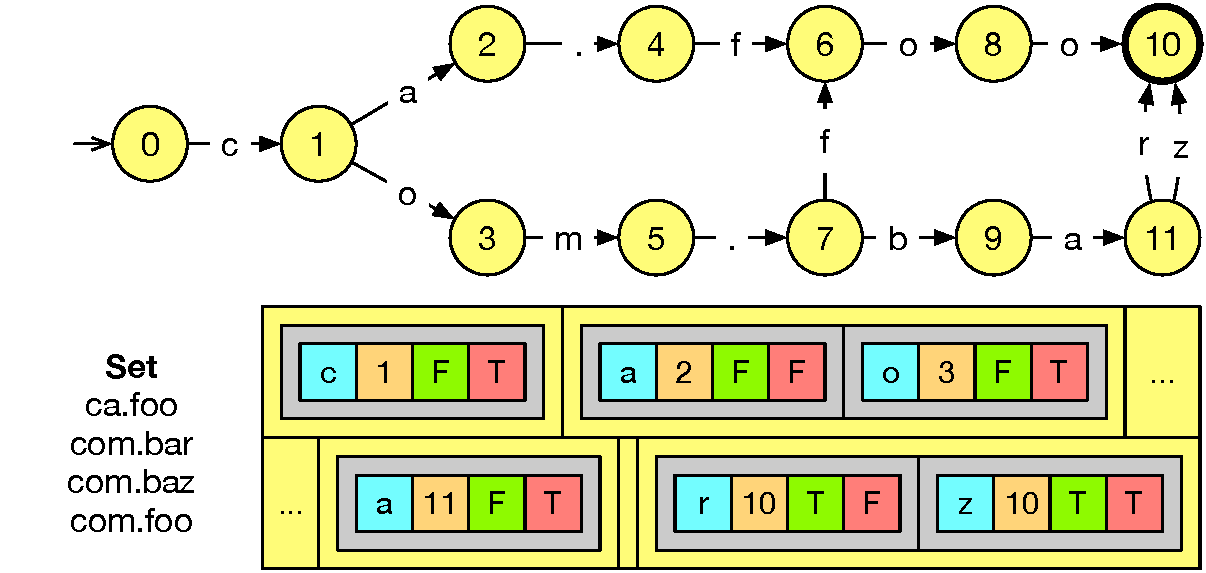
\includegraphics[width=\linewidth]{fig/dafsa}
  \caption{A simple \ac{dafsa} with one-character transitions, along with the
    set of strings it represents and its succinct representation as a vector of
    variable-length bitstrings. In this representation, each edge (gray)
    consists of a label (blue) and next state (orange), along with flags
  indicating whether the next state is an accept state (green) and whether the
edge is the last one outgoing from this state (red).}
  \label{fig:dafsa}
\end{figure}

In our log aggregator prototype, we ultimately chose to represent the signaling
set as a data structure known as a \emph{\acf{dafsa}}, which succinctly stores a
set of strings, supports efficient membership queries in this set, and supports 
efficient, compact construction~\cite{daciuk2000incremental}. As shown
in \autoref{fig:dafsa}, \iac{dafsa} takes advantage of both common prefixes and
suffixes that appear in a set of strings; since such patterns are frequent in a
large set of domain names, much of the redundancy in \httpsset can be removed with this
approach. Additionally, \acp{dafsa} can also be represented succinctly, using an
approach we summarize below~\cite{daciuk2012smaller}. Given the characteristics
of our input set as described in \autoref{sec:evaluation:implementation}, we
make an additional design change, \emph{path compaction},
to our \ac{dafsa} representation that further reduces its size.

\paragraph{Formal \ac{dafsa} Definition}

To precisely describe these changes, we begin by presenting a formal framework
to describe \acp{dafsa}. Formally, \iac{dafsa} is a tuple $(\symbols, \states,
\initstate, \transfunc, \finalstates)$ where
\begin{inparaenum}
\item \symbols is a set of possible \emph{input symbols},
\item \states is a set of \emph{states},
\item \initstate is an \emph{initial state} where $\initstate \in \states$,
\item $\transfunc: \states \times \symbols \to \states$ is a partial function
  called the \emph{state transition function} that maps a state-symbol pair to a
  new state, and
\item \finalstates is a set of \emph{accept states} where $\finalstates
  \subseteq \states$.
\end{inparaenum}
The \ac{dafsa} also has the restriction that the state transition function is
\emph{acyclic}, that is, there is no sequence of states and symbols $(s_1,
\ldots, s_n), (\sigma_1, \ldots, \sigma_n)$ where $\transfunc(s_i, \sigma_i) =
s_{i+1}$ for each $i$ where $1 \le i < n$ and $\transfunc(s_n, \sigma_n) = s_1$.

We represent queries to the signaling set within the \ac{dafsa} as follows: let
\states contain $\policy$ unique symbols $\multicertsymbol_\policy$ not present in \httpsset. 
Then, if there exists a sequence of
states and symbols $(s_0, \ldots, s_n), (\sigma_1, \ldots, \sigma_n)$ that
satisfies
\begin{inparaenum}
\item $\transfunc(s_i, \sigma_{i+1}) = s_{i+1}$ for each $i$ where $0 \le i < n$,
\item $\sigma_1 \| \dots \| \sigma_{n-1} = \hostname$, 
\item $\sigma_n = \multicertsymbol_\policy$, and
\item $s_n \in \finalstates$,
\end{inparaenum}
we say that $\query(\hostname) = \multicert(\policy)$.
Otherwise, if
\begin{inparaenum}
\item $\transfunc(s_i, \sigma_{i+1}) = s_{i+1}$ for each $i$ where $0 \le i < n$,
\item $\sigma_1 \| \dots \| \sigma_{n} = \hostname$, and
\item $s_n \in \finalstates$,
\end{inparaenum}
then $\query(\hostname) = \onecert$. Otherwise, $\query(\hostname) = \nohttps$.

\paragraph{\ac{dafsa} Representation}

We begin by building the \ac{dafsa} as described in previous
work~\cite{daciuk2000incremental}. Though this previous work assumes transitions
based on a single character, we consider the possibility of multi-character
symbols and thus our symbol set $\symbolstrings = \bigcup_{i=0}^{253}
\symbols^i$, where \symbols is the set of all ASCII characters allowed in domain
names.\footnote{Recall that DNS names can be a maximum of 253 characters.}

We succinctly represent this \ac{dafsa} as a bitvector by following the
high-level approach of previous work~\cite{daciuk2012smaller}. Intuitively, we
represent the \ac{dafsa} as a sequence of state encodings, which mostly consist
of outgoing transition encodings. By our definition of \transfunc, for a state
$s$, if $\transfunc(s, \sigma) = t$, then each outgoing transition must be
represented by an encoding of the label $\sigma$ and the destination state $t$.
We observe that in this construction, the overall number of outgoing
transitions, as well as the size of the representation of each transition's
label and destination state, strongly influence the size of the final bitvector.
We thus focus on leveraging patterns in the underlying data to minimize the size
of the \ac{dafsa} representation.

\paragraph{Path Compaction}

\begin{figure}
  \centering
  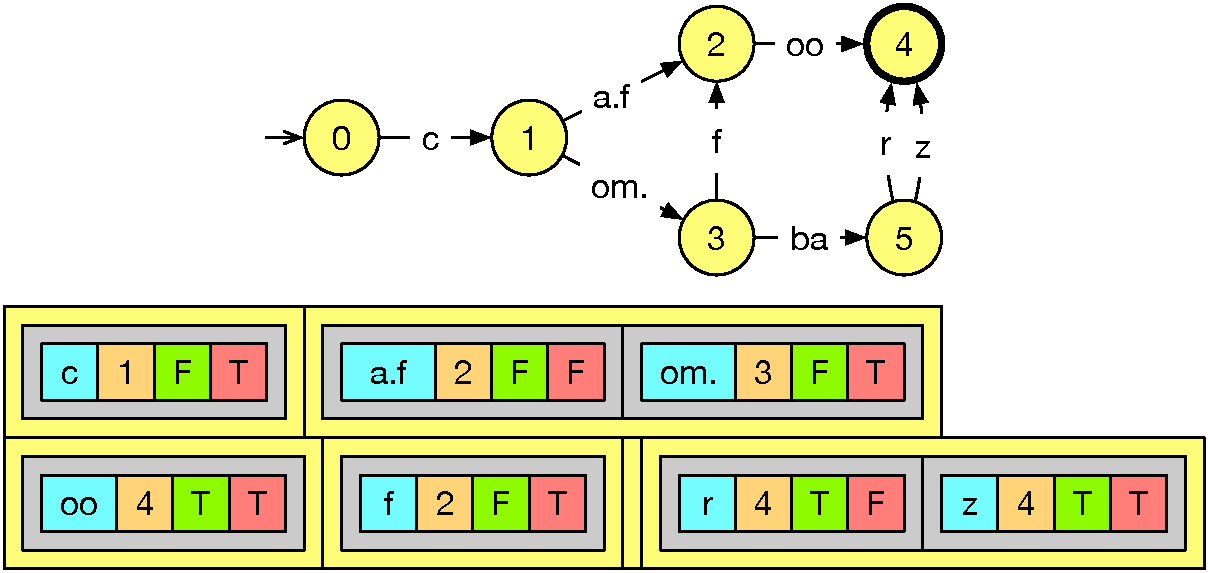
\includegraphics[width=\linewidth]{fig/dafsa_compact}
  \caption{The \ac{dafsa} from \autoref{fig:dafsa} with its long edges
  compacted. The binary representation is more succinct than its counterpart.}
  \label{fig:dafsa_compact}
\end{figure}

We extend the design of prior work with \emph{path compaction}, which
minimizes the \ac{dafsa} representation by reducing the overall number of
transitions. Intuitively, path compaction removes a connected set of states from
the \ac{dafsa} and replaces transitions into or out of this set with transitions
equivalent to paths through the set. As we formalize below, we can model this
process as the transformation of one \ac{dafsa} into another and use this model
to determine how we should select a set of nodes to ensure a minimal \ac{dafsa}
representation.

Given \iac{dafsa} $(\symbols, \states, \initstate, \transfunc, \finalstates)$,
we define a \emph{walk} between $s_1$ and $s_m$ to be a sequence of alternating
states in \states and symbols in \symbols, written $(s_1, \sigma_1, \ldots,
s_m)$, where for all $i$ where $1 \le i < m$, either $\transfunc(s_i, \sigma_i)
= s_{i+1}$ or $\transfunc(s_{i+1}, \sigma_i) = s_i$ (i.e., a walk treats the DAFSA's
edges as undirected).
A walk where
$\transfunc(s_i, \sigma_i) = s_{i+1}$ for all $i$ where $1 \le i < m$ is called
a \emph{path} from $s_1$ to $s_m$. We say that a set of states $\stateset
\subseteq \states$ is a \emph{connected component} if either $\stateset
\subseteq \finalstates$ or $\stateset \cap \finalstates = \varnothing$, and for
any two states $t, u \in \stateset$, there exists a walk between $t$ and $u$.
The \emph{upstream states} of a connected component \stateset, written
\upstream{\stateset}, is the set of all states $s \in \states \setminus
\stateset$ for which there exists a state $t \in \stateset$ and a symbol
$\sigma$ where $\transfunc(s, \sigma) = t$. The \emph{downstream states} of
\stateset, written \downstream{\stateset}, is the set of all states $s \in
\states \setminus \stateset$ for which there exists a state $t \in \stateset$
and a symbol $\sigma$ where $\transfunc(t, \sigma) = s$. A path \emph{through} a
connected component \stateset is a path $(s_1, \sigma_1, \ldots, s_m)$ where
$s_1 \in \upstream{\stateset}$, for all $i$ where $1 < i < m$, $s_i \in
\stateset$, and $s_m \in \downstream{\stateset}$.

Path compaction consists of repeatedly
\begin{inparaenum}
\item selecting a connected component \stateset within the \ac{dafsa},
\item calculating the estimated reduction in representation size from compacting
  the paths through \stateset, and
\item if the change reduces the size of the \ac{dafsa} representation, removing
  these states from \states and replacing the paths through \stateset with an
  equivalent set of transitions.
\end{inparaenum}
Specifically, when removing \stateset, we transform the \ac{dafsa} $(\symbols,
\states, \initstate, \transfunc, \finalstates)$ to $(\symbols, \states \setminus
\stateset, \initstate, \transfunc', \finalstates)$, where for all paths $(s_1,
\sigma_1, \ldots, s_m)$ through \stateset, $\transfunc'(s_1, \sigma_1 \| \dots \|
\sigma_{m-1}) = s_m$.

Our goal is to select components that result in the greatest reduction in size.
To determine the size reduction of removing a connected component, we must
consider both the reduction in the number of edges in the \ac{dafsa} as well as
any changes to the symbol and destination state entropy, as removing a component
would cause the distributions underlying these values to change. To quantify
this change, we define several helpful variables.

For a set $X \subseteq\states$, let \numtrans{X} denote the set of transitions
that start or end in $X$, that is, the number of triples $(s, t, \sigma)$ where
$\transfunc(s, \sigma) = t$ and $s$ or $t$ (or both) is in $X$. For a connected
component $C$, let \numpaths{C} denote the set of paths through $C$. Then the
change in the number of edges by removing $C$ through path compaction is
$|\numpaths{C}| - |\numtrans{C}|$. By examining the distribution of symbols in
\numtrans{S} and \numtrans{C}, as well as the concatenated symbols in
\numpaths{C} (which we can find via depth-first search from \upstream{C}), we
can compute the change in entropy in symbols and similarly for destination
states, which we write as \symboldh and \destdh, respectively. If we know the
original entropies \symbolh and \desth, then we can compute the difference in
size between the two \acp{dafsa} as
\begin{equation}
  |\numtrans{S}|\left(\symboldh + \destdh\right) + \left(|\numpaths{C}| -
  |\numtrans{C}|\right)(\symbolh + \symboldh + \desth + \destdh)
\end{equation}
and only remove $C$ if this quantity is negative.

We found several classes of components that, for our underlying set of domain
names, provided substantial reductions in the size of the \ac{dafsa}
representation. The first was to select what we call \emph{isolated paths}, that
is, paths of the form $(s_1, \sigma_1, \ldots, s_m)$ where for all $i$ such that
$1 < i < m$, $s_i$ only had one incoming and one outgoing transition. 
Using techniques from prior work~\cite{daciuk2000incremental} to build the \ac{dafsa} 
results in a significant number of isolated paths.
Hence performing path compaction on all such paths
results in a size savings of nearly 10\% of the original \ac{dafsa} size.
We also found that selecting a constant $\alpha$ and then selecting components
consisting entirely of states that had one incoming transition and $\alpha$
outgoing transitions (or vice versa) yielded more modest but still nontrivial
size reductions for $\alpha = 2$ and $\alpha = 3$.

\subsection{Building the \ac{name} Policy Database}
\label{sec:design:policy}

The policy database represents a binding between a name and a policy, that
is, the number of independent certificate chains that a client
should expect during a handshake with a server corresponding to the name.
To construct and maintain this database, each log aggregator must keep track of
the certificates and chains active for a domain at any given time. The log
aggregators again rely on the data used to build the signaling set.
%from public sources for this information,
%which includes the data used to build the signaling set, as well as certificate
%chains observed by public logs.

\begin{figure}
  \centering
  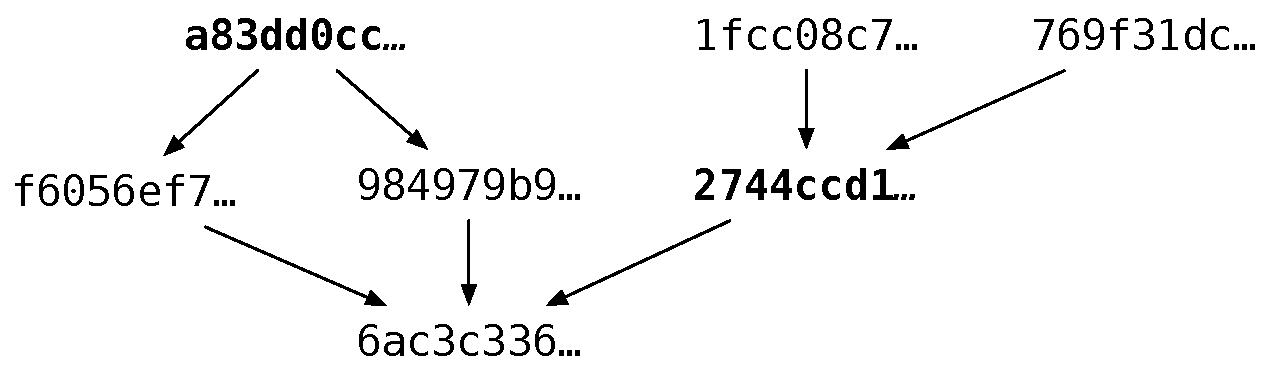
\includegraphics[width=\linewidth]{fig/chain}
  \caption{Sample certificate fingerprint graph. An arrow from A to B indicates
    that a certificate with fingerprint A is the authority public key for a
    certificate with fingerprint B. Though the leaf certificate
  $\texttt{6ac3c336}\ldots$ has four chains, only two of the chains are
independent.}
  \label{fig:chain}
\end{figure}

A log aggregator uses this data to maintain an internal database with
(many-to-many) maps of
\begin{inparaenum}
\item certificates to names,
\item certificates to public keys, and
\item certificates to chains.
\end{inparaenum}
Regular updates to this database (described in \autoref{sec:design:signaling})
ensure that the log aggregator has a list of currently valid certificates. The
log aggregator can then use the database to construct a mapping of names to
policies. Specifically, the aggregator creates a graph of certificate
fingerprints as shown in \autoref{fig:chain}, and computes the \emph{policy
value}, the minimum number of \ac{ca} public keys that must be compromised to
fraudulently issue this certificate. The policy value can be computed using a
straightforward approach (e.g., computing a minimal vertex separator), allowing
the log aggregator to easily construct a mapping of certificate fingerprints to
policy values. The log aggregator can then perform a series of simple join
operations to map each name to the maximum policy number associated with a
certificate containing the name.

The log aggregator constructs this name-to-policy mapping each time it receives
data from public sources (recall from \autoref{sec:design:signaling} that this
occurs at regular, scheduled intervals). Once it has created the mapping, the log
aggregator certifies the name--policy-value pairs in this mapping by
timestamping and signing them.\footnote{For efficiency, the log aggregator can
  sign a subset of pairs each day, and have each client consider a signature
  valid for multiple update intervals. For example, the log aggregator could
  sign a third of the pairs each day, and clients could treat a signed,
timestamp pair as valid for at least three days.}

With the policy databases of the log aggregators, a domain can provide the
information necessary for clients to establish the domain's authoritative public
key in the improved \ac{pki}. The domain periodically downloads the latest
\emph{policy proofs}, which are signed and timestamped name-policy pairs, from
each of the log aggregators. For a name \hostname, a policy value \policy, a
timestamp \timestamp, and a log aggregator \logagg, we specify the policy proof
to be
\begin{equation}
  \policyproof(\logagg, \hostname, \policy, \timestamp) = \left\{\timestamp,
  \pk_{\logagg}, \signature(\pk_{\logagg}^{-1}, \hostname \concat \policy
\concat \timestamp)\right\}
\end{equation}
where $\pk_{\logagg}$ and $\pk_{\logagg}^{-1}$ denote respectively the public
and private keys of \logagg, and $\signature(K, m)$ denotes a signature on $m$
with private key $K$. The domain keeps these proofs for use in the handshake
described below.

\subsection{Connection Establishment}
\label{sec:design:handshake}

To establish a connection to a domain, a client first queries the 
signaling set for the domain's name.
%Due to the way that querying occurs in the
%\ac{dafsa}-based implementation of the signaling set, the client can observe the
%state transitions in the \ac{dafsa} and, if the symbols making up the domain
%name lead to a state that is not an accept state, the client can supply
%\multicertsymbol to determine whether that transitions to an accept state (and
%hence the domain has a policy value greater than 1). 
If this query returns
\onecert or $\multicert(n)$, then the client performs the \ac{name}-extended
TLS handshake to establish a connection with the domain.

The \ac{name}-extended TLS handshake protocol allows a client to verify a domain's
authoritative public key. The \ac{tls} handshake protocol~\cite{rfc5246}
provides support for open-ended extensions (implemented in cryptographic
libraries), and thus we designed our protocol as an extension within the
existing \ac{tls} handshake. During the initial ClientHello message, the client
includes a \ac{name} extension message, which consists of a single integer
\numlas, indicating the number of policy proofs that the domain should send back.
%We assume that a reasonable maximum value for \numlas is enforced; for example,
%a domain may abort the handshake if \numlas is beyond some acceptable maximum.
In an initial deployment, we expect that typically $k=1$,
but allowing the use of larger values for $k$ provides resilience
against compromised log aggregators.

The domain then sends back a ServerHello message which contains \numlas
recent policy proofs from \numlas distinct log aggregators, as well as \numlas
certificate chains, which allows the client to verify the domain's policy
value and the certificate chains that back this value.
In more detail, a domain with hostname
\hostname and policy value \policy selects a set of log aggregators
$\{\logagg_1, \ldots, \logagg_\numlas\}$ and sends back
in the ServerHello extension message:
\begin{equation}
  \{\policyproof(\logagg_1, \hostname, \policy, \timestamp_1), \ldots,
  \policyproof(\logagg_\numlas, \hostname, \policy, \timestamp_\numlas),
\certchain_1, \ldots, \certchain_{\policy - 1}\}
\end{equation}
where $\timestamp_i$ is the timestamp of the policy proof from $\logagg_i$ and
$\certchain_j$ is a certificate chain for \hostname. In the extension message,
the domain only sends $\policy - 1$ certificate chains because the remaining
chain will be sent in the ServerCertificate message of the TLS handshake.

The client then checks that
\begin{inparaenum}
\item the signature on each policy proof is valid,
\item the timestamp for each policy proof is sufficiently recent,
\item the name in each policy proof is the domain's name,
\item the policy value for each policy is one more than the number of
  certificate chains sent in the domain's extension message, and
\item each certificate chain is valid as specified in the X.509v3
  standard~\cite{rfc5280}.
\end{inparaenum}
If the above checks pass, the client can then continue with the standard TLS
handshake, which requires the client to verify an additional certificate chain
in the ServerCertificate message and perform all other checks required by the
\ac{tls} handshake protocol.


\subsection{Bootstrapping Advanced Policies}
\label{sec:design:bootstrapping}

Once an authoritative public key for a domain has been established through the
\ac{name} handshake, signatures made by the corresponding private key can be
used to verify the binding between a domain and a richer set of policies. For
example, in systems such as ARPKI~\cite{basin2014arpki} and
PoliCert~\cite{szalachowski2014policert}, these policies can specify a set of
\acp{ca} that are authorized to issue certificate for the domain, or even make
the domain a \ac{ca} for itself by pinning specific public keys to the domain.
In this way, the authoritative public key established in \ac{name} can be used
to bootstrap confidence in these advanced policies while preventing downgrades
to the old \ac{pki}.

This bootstrapping approach obviates the need for logs to directly store the
policies, which can be quite large in these previously proposed systems.
Moreover, in \ac{name}, this bootstrapping can take place at any time during
deployment, which means that in the case of a lost or compromised private key,
a domain can simply obtain \policy + 1 new, independent certificate chains.
This contrasts with previous proposals, which often rely on heavyweight
processes that involve manual \ac{ca} intervention.

The authoritative public key can also be used directly, as
a way of providing clients with more confidence in the current \ac{pki}.
